\chapter{Limitantes}

\section{O que são Bounds?}
Dentro do contexto de algoritmo Branch and Bounds, os Bounds são estimativas que fazemos utilizando informações conhecidas do problema, com o intuito de criar um intervalo limitado superiormente e inferiormente no qual temos certeza que o ótimo resultado está contido. Sendo assim, possuímos um Upper Bound (UB) que limita nossa solução superiormente, ou seja, a solução ótima que buscamos é menor ou igual ao UB, e também possuímos um Lower Bound (LB) que limita nossa solução inferiormente, ou seja, nossa solução ótima é maior ou igual ao LB. Os limitantes não são fixos e a cada iteração do Bnb eles são recalculados com o intuito de deixar nossa 
\section{Upper Bounds e Lower Bounds}

Vários Bounds nos foram apresentados no 

\subsection{De Permutações para Grafos}

Em nosso algoritmo exato, para a construção de um dos limitantes, precisaremos modelar uma nova estrutura da qual será mais eficiente extrair informações que otimizaram o algoritmo. Esta estrutura é um grafo, para construirmos o grafo $G(\pi)$ onde $\pi$ é uma permutação qualquer, cada breakpoint [$\pi_i, \pi_{i+1}$] de $\pi$ será um vértice em G. E cada aresta será criada unindo dois vértices em G a partir das seguintes regras:\\

1º Se o par de vértices (breakpoints) podem ser removidos por uma única reversão. \\

2º Se o par de vértices (breakpoints) podem ser removidos por uma sequencia de reversões que removem 2 BP. \\


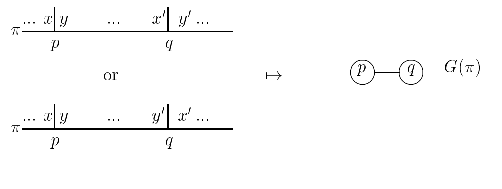
\includegraphics{Imagens/grafo exemplo.png}


\subsection{Matching Máximo}
Um matching (= emparelhamento) num grafo G não-dirigido é um conjunto E de arestas dotado da seguinte propriedade: todo vértice de G incide em no máximo um elemento de E.  (Um laço não pode fazer parte de um emparelhamento porque incide duas vezes em um mesmo vértice.)

Um emparelhamento $M$ é máximo se não existe um emparelhamento $M'$ tal que $\|M'\| > \|M\|$.  Além disso, um emparelhamento M é maximal se não existe um emparelhamento M' do qual M faça parte própria (portanto, $M$ é maximal se não existe aresta a fora de $M$ tal que $M+{a}$ também é um emparelhamento).

Com esta nova definição, sendo o matching o conjunto de arestas vértices-disjuntas, onde cada aresta modela uma reversão e remove 2 BP. Denotaremos por m o número de vértices da cardinalidade máxima do matching de $G(\pi)$.

A pergunta agora é, quantas reversões são necessárias para remover os $\phi(\pi) - m$ BP restantes. O melhor que podemos performar é uma 1-reversão que configura uma 2-reversão para o próximo passo; Não é possível fazer uma 2 reversão novamente pois uma reversão só afeta 2 BP, e com isso a 3ª reversão só poderia ser feita se já estivesse disponível desde o começo, porém se isso fosse verdade ela já estaria contida em M que é a cardinalidade máxima. Logo a nossa melhor opção está é remover 3 BP em 2 passos, com isso obtemos o seguinte \textbf{Lower Bound}:
    
\begin{center}
$[((1/2) * M) + 2/3 (\phi(\pi)) - M)]$    
\end{center}












\subsection{Programação Linear}
- Permutação dirigido
- Hyper grafo
- 


Na execução, dada uma permutação como entrada, enquanto a permutação possuir breakpoints o algoritmo executa, é incrementado em 1 a quantidade de reversões aplicadas , a partir daí é aplicada uma reversão que remova o máximo de breakpoints possíveis (estratégia gulosa), após isso a reversão aplicado é incluída na lista solução que está sendo construída. Esta execução é feita em loop sendo a condição de parada o fim dos breakpoints na permutação de entrada. Por usar a estratégia gulosa, ele busca sempre a reversão que possa ser o melhor candidato, em casos que existam empate entre reversões que removam 1 BP, o desempate é dado pela preferência em utilizar reversões que deixam substring decrescente (SD), tomando como base o  lema 4.1.\\


A maneira que este algoritmo foi descrito por Kececioglu nos da algumas garantias como veremos, que podemos ordenar uma permutação com $k$ BP, fazendo no máximo $k$ reversões.

(Contar o que o algoritmo faz, não necessariamente como ele faz )

(Não se sabia sobre a questão da dificuldade do algoritmo, e o que foi aprendido sobre essa questão)